%%%% Don't include, has been split into other files..
\section{Refactoring} \label{sec:s4_refactoring}
\subsection{Class Architecture}
In order to describe the structure design of the HotMap server, the UML v2.5 standard is used to express how the class hierarchy was designed. UML is a well known modelling language, for visualising software system designs in order to more easily describe the static structure of a software system.
Therefore a UML class diagram is used for describing the model layer of the HotMap server.

\jenote{Flyt det her op til sin egen subsection under refactoring}
Mixin is a language dependent functionality that we use in our application, which allows a class \emph{A} to contain methods from other classes or interfaces without having \emph{A} be a specialisation of these other classes or traits. How class \emph{A} gain access to those methods through mixin is defined by the language. 

Scala does not have interfaces, but instead uses traits. These are similar but allow for default implementation of methods within the trait. When concrete classes extends traits, it is called a realisation of that trait, which in UML is indicated by a dashed arrow from the class to the interfaces. In Scala, traits can also be instantiated if all of its instance variables and methods have default implementations. Scala only allows traits to be mixed into classes or other traits.

In Scala, type aliases of mixin types are used to denote a class or trait with a trait mixed into it. As an example of this we have on \cref{fig:class} that type \emph{Point} is an alias for any type which realises the trait \emph{Coordinate} mixed with the trait \emph{Weight}. UML cannot represent mixin, so it was chosen to show this by drawing a realisation arrow with a mixin stereotype from the alias to the mixed type. Stereotypes are denoted by some text surrounded with \emph{<<} and \emph{>>} above the arrow.

\subsubsection{Class Diagram}

This section will explain the most notable classes illustrated in \cref{fig:class} and its relations.

The \emph{Coordinate} trait models a geographic location on the earth. Because many functions are dealing with objects that can have coordinates, we can let these objects implement the \emph{Coordinate} trait, and thereby write these functions in a polymorphic way. One such object is the \emph{Position} class, which is essentially a coordinate for a person at a given time. \emph{ConfidencePosition} is designed to have the same structure as positions received from the aSTEP server, so when hopMap request position data a list of \emph{ConfidencePosition} will be returned. A \emph{ConfidencePosition} therefor also includes information about the certainty of a position, called Confidence as shown on \cref{fig:class}. This confidence is a distance which the position at most is offset from. \emph{ConfidencePosition} also has a \emph{lastLocatedTime} which is a time stamp for when the position was recorded by the aSTEP server.


The \emph{Person} class is a abstract class, defining methods which should be implemented in specialisations of this class, in order to enforce code reuse and consistency. The class contains the person's history of positions as an iterateable collection of the generic type \emph{T}. The generic type parameter \emph{T} is bounded to be a class implementing \emph{Coordinate}, denoted by \emph{T < Coordinate}. This prevents any specialisation of \emph{Person} from having a history of positions that is not a collection of \emph{Coordinate}s. \emph{T} is in a contravariant position, denoted by \emph{-T}, permitting specialisations of the \emph{Person} class to use a specialisation of \emph{T}. Contravariance allows the \emph{Person} class to have methods that takes an input of type \emph{T}, but excludes the class from defining methods which returns a \emph{T}. The most important method in the \emph{Person} class is \emph{movePerson}, which takes a \emph{T} and a \emph{DateTime} as parameters. Here the parameter of type \emph{T} is the location the person should be moved to, and the DateTime parameter is the time where the person arrived at the location. This method updates a person's history of positions to include the new position. Upon updating a person's history of positions, positions older than \emph{x} is removed from the person, where \emph{x} is a constant defined for all persons. To calculate a person's velocity and heading direction this history of positions is essential. 

\emph{Area} is an abstract class representing a geographical area on a map. The most important method in the class that should implement is the function \emph{isWithinArea}. There are two versions of the function. One takes a coordinate and returns a boolean denoting weather this coordinate is within the area. The other takes a iterateable collection of generic types T and a function that goes from T to a coordinate. It returns a new filtered iterateable collection of T only consisting of the objects within the area.

\emph{PopulatedArea} is a class mixing an area with a population. The responsibility of this class is to cache and update the positions of people within its area. The two main things this class must be able to do, is to update the positions of the people within it and be able to find the positions of all the people within it given a time. Since this is the class responsible for caching of peoples positions it also hold the policy of when to throw away positions and to extension the people holding them, if they for instance leave the area, and are no more relevant. It is therefore also responsible for any misses in its people position cache, and request the aSTEP for these positions. Since it is people themselves that throw away their positions this class must know about the policy of the person given to it, in order to be able to know when to request new positions from the aSTEP core and add these to the person. This class, together with the person class, hold the policy on how that given a specific time stamp, finding the position closest to this time stamp for each person, and judging when there is one close enough.

\begin{sidewaysfigure}[htbp]
\centering
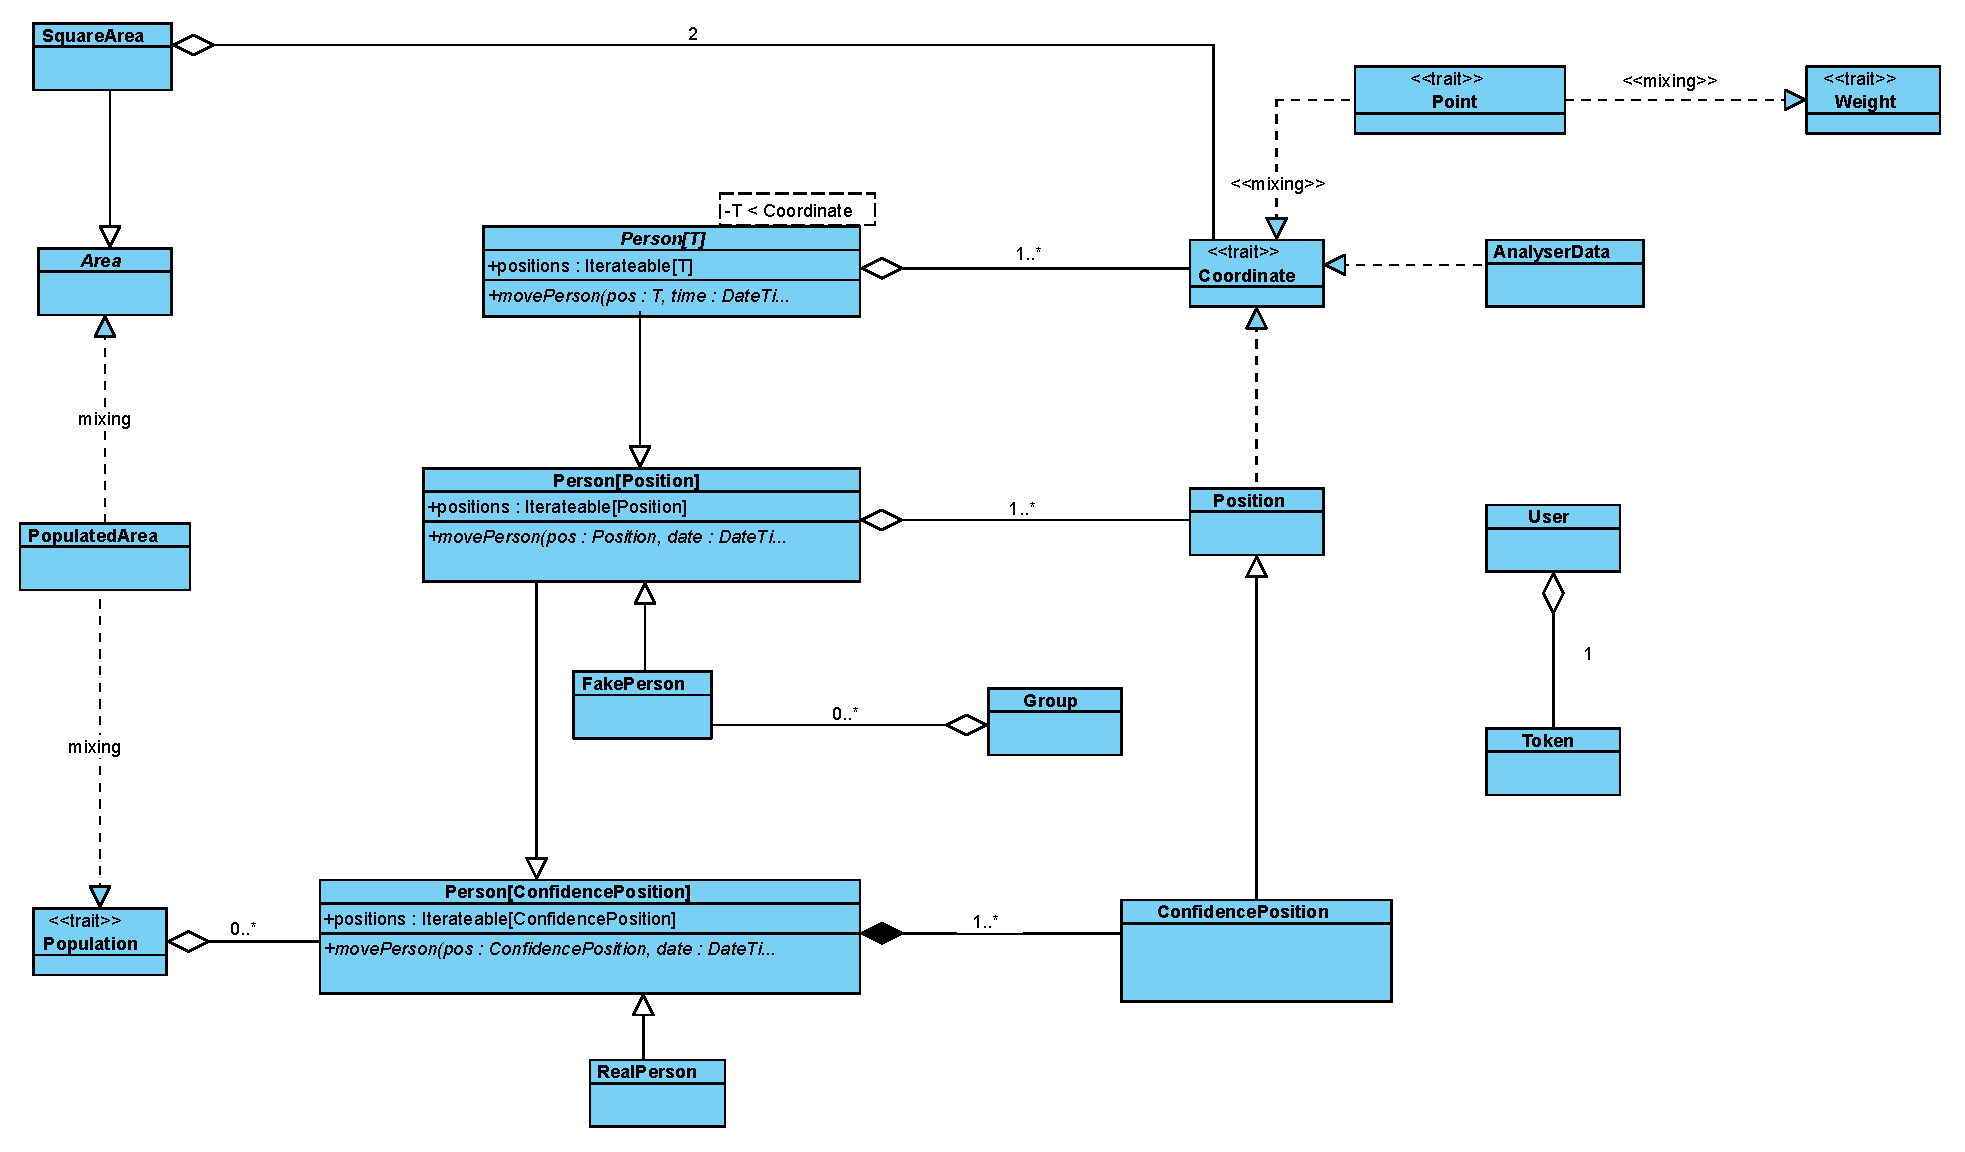
\includegraphics[width=\linewidth]{figures/class.eps}
\caption{Class diagram.}
\label{fig:class}
\end{sidewaysfigure}

\subsection{Implementation of Asynchronous Analysis}
\label{sub:implementation_of_asynchronous_analysis}

As described in \cref{sub:Asynchronous_Analysis} the amount of calculations required can be reduced by analysing location data asynchronously from user requests, storing completed analyses. We assume that users will primarily monitor real-time crowd factors, therefore we will focus on optimising the real-time analysis.

This was implemented using an infinite loop running on another thread. This thread fetches and analyses position data from the aSTEP core. Completed analyses from this thread are stored in a global variable. When a user requests crowd factors the request handler will respond with data obtained from this global variable. 

There is one thread which writes data to the global variable, and potentially one thread per user reading data from this global variable. The global variable is a pointer to the result of the latest completed analysis. When the analysis of new data is completed, this pointer is changed atomically, in order to prevent race conditions. 

The infinite loop is repeated at most once per 5 seconds. In the case that an iteration of the loop takes longer than 5 seconds to complete, the next iteration will not start until the current iteration has completed. The 5 second limitation corresponds to the frequency at which the aSTEP core can supply updated data. One iteration of the loop consists of the following five stages: 

\begin{enumerate}
    \item \textbf{Process the position data:} At this stage all the fetched positions are associated with the corresponding person, based on a id received together with every position. This id identifies a single Wi-Fi device. Afterwards the method \emph{movePerson} is called for every instance of the class \emph{Person}, with the corresponding new position as parameter, in order to add this position to a persons history.
    \item \textbf{Fetch position data:} This stage fetches position data from the aSTEP core.
    \item \textbf{Calculate analysis data:} The purpose of this stage is to calculate the list of \emph{AnalyserData} for each \emph{Area}. This involves calculating all peoples heading direction and velocity, and encapsulate this in an instance of the class \emph{AnalyserData}.
    \item \textbf{Analysis:} This stages analyses the data from the last stage, estimating the crowd factors of each \emph{Area}.
    \item \textbf{JSON Conversion:} At the last stage the result of the analysis is converted into JSON format, which is then stored in the global variable used for user requests. 
\end{enumerate}

In summary, this implementation ensures that the data analysis is not performed for all users requesting real-time information, which improves the performance of the server. It also improves client side performance, as handling requests of analysed data takes less time. Another advantage of this implementation is that multiple users monitoring real-time crowd conditions will be shown the exact same information.
